\documentclass[border=6pt]{standalone}
% Shared preamble for web figures.  Each figure is a standalone .tex that
% \input's this file; scripts/make-figures.sh turns it into an SVG.
% Handouts pull the same file with \fig{Unit_X/<name>}.
\usepackage[T1]{fontenc}
\usepackage{helvet}
\renewcommand{\familydefault}{\sfdefault}
\usepackage{amsmath}
\usepackage{tikz}
\usetikzlibrary{arrows.meta,positioning,calc,shapes.symbols,shapes.geometric}

% Who makes the rules is the point of most diagrams in this book, so the
% colors mean the same thing everywhere: blue is a person, orange is the
% computer, green is an answer, pink is the human brain.
\definecolor{person}{HTML}{2C6FAE}
\definecolor{machine}{HTML}{D35400}
\definecolor{result}{HTML}{1E8449}
\definecolor{brainpink}{HTML}{C2185B}
\definecolor{ink}{HTML}{2C3E50}

\tikzset{
  doodle/.style={line width=1.5pt, line cap=round, line join=round, draw=ink},
  box/.style={draw, rounded corners=5pt, line width=1.1pt, align=center,
              inner sep=7pt, minimum height=1.0cm, font=\small},
  personbox/.style={box, draw=person, fill=person!10},
  machinebox/.style={box, draw=machine, fill=machine!10},
  resultbox/.style={box, draw=result, fill=result!10},
  plainbox/.style={box, draw=ink!70, fill=ink!4},
  flow/.style={-{Stealth[length=8pt]}, line width=1.4pt, draw=ink},
}

\begin{document}
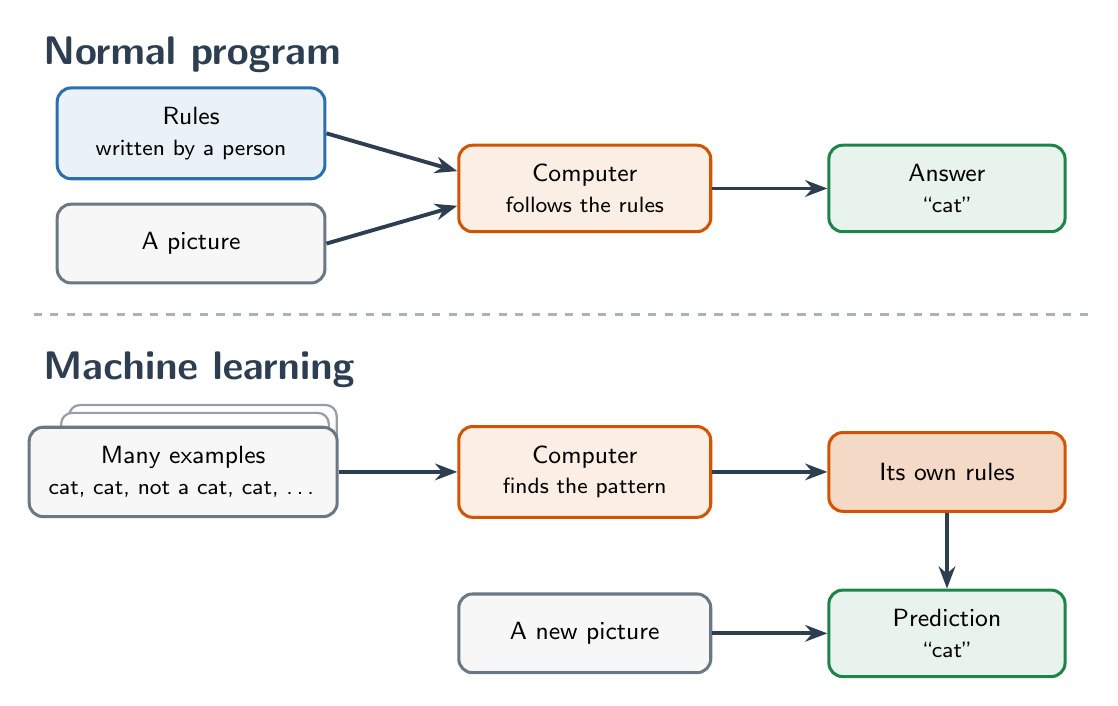
\begin{tikzpicture}
% Top: a person writes the rules.  Bottom: the computer makes its own rules
% from examples, then uses them on a new picture.

% ---------- Normal program ----------
\node[anchor=west, font=\Large\bfseries, text=ink] at (-0.4,5.75) {Normal program};
\node[personbox, minimum width=3.4cm] (r1) at (1.6,4.75) {Rules\\{\footnotesize written by a person}};
\node[plainbox, minimum width=3.4cm] (i1) at (1.6,3.35) {A picture};
\node[machinebox, minimum width=3.2cm] (c1) at (6.6,4.05) {Computer\\{\footnotesize follows the rules}};
\node[resultbox, minimum width=3.0cm] (a1) at (11.2,4.05) {Answer\\{\footnotesize ``cat''}};
\draw[flow] (r1.east) -- ($(c1.west)+(0,0.22)$);
\draw[flow] (i1.east) -- ($(c1.west)+(0,-0.22)$);
\draw[flow] (c1) -- (a1);

\draw[dashed, ink!40, line width=0.8pt] (-0.4,2.45) -- (13.0,2.45);

% ---------- Machine learning ----------
\node[anchor=west, font=\Large\bfseries, text=ink] at (-0.4,1.75) {Machine learning};
% a small stack of example cards behind the box
\draw[ink!50, fill=white, rounded corners=4pt, line width=0.8pt] (0.05,0.0) rectangle (3.45,1.3);
\draw[ink!50, fill=white, rounded corners=4pt, line width=0.8pt] (-0.05,-0.1) rectangle (3.35,1.2);
\node[plainbox, minimum width=3.4cm] (e2) at (1.5,0.45) {Many examples\\{\footnotesize cat, cat, not a cat, cat, \dots}};
\node[machinebox, minimum width=3.2cm] (c2) at (6.6,0.45) {Computer\\{\footnotesize finds the pattern}};
\node[machinebox, fill=machine!22, minimum width=3.0cm] (r2) at (11.2,0.45) {Its own rules};
\draw[flow] (e2.east) -- (c2);
\draw[flow] (c2) -- (r2);

\node[plainbox, minimum width=3.2cm] (n2) at (6.6,-1.6) {A new picture};
\node[resultbox, minimum width=3.0cm] (p2) at (11.2,-1.6) {Prediction\\{\footnotesize ``cat''}};
\draw[flow] (r2) -- (p2);
\draw[flow] (n2) -- (p2);
\end{tikzpicture}
\end{document}
